\section{Experiments}\label{sec:experiments}

Everything in this section that is a number was measured on the CPU with the project code and fixed seeds, on small samples, and
every sample size is stated. All measured results are simulation-driven. No language model has been trained or evaluated: no SFT or GRPO checkpoint exists and no model arm has been scored. The frontier zero-shot and harness arms are replays of saved answers from \texttt{data/kaggle\_datasets/thermo-agent-eval-replays/}, scored through the same verifiers. The model results and ablations (\cref{sec:modelresults,sec:ablations}) are skeletons whose cells are pending, and every protocol value below is pre-registered rather than measured. Datagen is not complete (\cref{sec:datagenstatus}), so by Reza's directive of 2026-11-19 training has not started. The frozen test set is \texttt{data/heldout\_v2}; the 214-id \texttt{data/heldout} is the dev set used for tuning only.

\subsection{Pre-registered protocol}\label{sec:protocol}

\paragraph{Models and harness.}
We evaluate the arms of decision F4. (i) Base Qwen3.5-4B and Qwen3.5-9B; (ii) our SFT checkpoint; (iii) our GRPO checkpoints at $k=4,8,16$, each from the merged SFT policy. Each of these appears in two modes: Z (plain prompt, no tools) and H (compact harness, tools and memory). (iv) Frontier zero-shot (Z) and frontier harness (H) arms, which are replays of saved answers from \texttt{data/kaggle\_datasets/thermo-agent-eval-replays/} through the same verifiers and prompt rows; a replay is evidence for that saved answer set only. (v) Other-LLM stand-in arms, plus the non-model baselines of \cref{sec:baselines}. The old \texttt{sft none} guard is replaced by this table; the two modes of a given model are scored on identical rows, so the harness effect is a paired comparison. Every arm sees the same rows of the frozen \texttt{heldout\_v2} test set and the same answer budget. Frontier models are reached through Kaggle's model access (not a local API); their saved answers are replayed, and Kaggle reports the token cost of each call. The mode and tool-access axes are recorded as columns in \cref{tab:comparison}. No arm has been scored yet; the SFT-tools-only versus SFT-mix comparison of decision F5 is deferred until the main table exists.

\paragraph{Decoding, attempts and budgets.}
Decoding is pre-registered as follows (all local arms identical). The primary condition is greedy decoding (\texttt{do\_sample=False}, repetition penalty 1.0, no presence penalty). A secondary pass@8 uses temperature 0.6, top-p 0.95, top-k 20, min-p 0 and seeds 0--7, again without repetition or presence penalties; these are Qwen's published thinking-mode precise-task settings (the general-chat presence penalty of 1.5 is rejected because structured output legitimately repeats unit tokens, ids and tool arguments). Frontier hosted models use provider defaults, which are recorded per run. The harness runs up to six tool rounds with at most eight tool calls; per-turn generation is capped at 4,096 new tokens, with a sequence gate of 8,192 tokens and over-gate rows dropped rather than truncated. Cost is counted in solver calls (Repair) or design evaluations (Design). Design also has an anytime protocol: the model is told the fuel of each valid design and may
refine, and we record the best gap to the reference after $b$ design evaluations, to compare with enumeration, random search and
enumerate-then-polish at equal budgets. None of these conditions has been run.

\paragraph{Metrics.}
Repair: success (the repaired plant is valid and serves the site), first-turn success, exact restoration on deducible faults, and mean solver calls. Design: valid share, share within 1\% of the reference, mean fuel gap, mean
evaluations. Audit: ranking score, validity of the change, gain and prediction score. Ledger repair: exactness, closure and the share of rows with all lines correct.

\paragraph{Statistics.}
Binary outcomes carry Wilson 95\% intervals \citep{wilson1927interval}. Two runs on the same examples are compared with an exact McNemar test for binary
metrics \citep{mcnemar1947}, and with a paired bootstrap interval plus a sign-flip permutation test for other metrics; all comparisons reported together are
Holm-corrected \citep{holm1979}. Per-example results are saved with each report. ThermoQA accuracy before and after training checks for forgetting.

\paragraph{Test set, dev set and tiers.}
The held-out test set is \texttt{data/heldout\_v2}, frozen before any model is scored; \texttt{data/heldout} (214 test ids) is the dev set and is used for tuning only, never reported as a test result. Within each task, rows are split into \texttt{easy}, \texttt{medium} and \texttt{hard} in equal thirds in both the training corpora and \texttt{heldout\_v2}; the tier is a real column derived from a documented per-task size measure (\texttt{thermo\_agent/synth/tiers.py}), never random and never a threshold tuned by the assistant. When a task's rows cannot be cut into exact thirds, the remainder goes to the higher tier and the manifest records the exact counts per task. The target is at least 85 rows per reported cell where a generator can reach it, with any merged cells documented explicitly. All of this is a pre-registered design: no cell has been scored.

\paragraph{Cost accounting and provenance.}
Three costs are reported separately and never merged into one score. Physics cost is solver calls (Repair) or design evaluations (Design); it is measured for every arm by the same evaluator. Model cost is the token count and the price that Kaggle Benchmarks reports for a frontier call (in nanodollars, summed per model in \texttt{reports/frontier\_ingest.json}), plus GPU-hours for our own training and inference. Data cost is the number of ground-truth plants, paraphrases, teacher attempts and accepted rows. Because frontier answers are static replays, their cost is charged once and reused across arms; the report states this instead of implying a fresh call per evaluation. Every result file carries the model id, harness mode, tool-access flag, seed, limit and sample size in its \texttt{meta} block, and the paper tables are generated from those files rather than transcribed.

\paragraph{Qualitative evidence.}
Figures are not hand-drawn illustrations. \Cref{fig:fig_trace_walkthrough} is regenerated from a deterministic selection of real traces -- a fault from the ground-truth corpus, a frontier interaction with recorded tool calls and reasoning (from the 32 accepted traces, replayed), a GRPO group (planned; none has been generated), and the comparison arms (planned) -- with the field schema and source files stored beside the examples. The selection rule is part of the generator, so the same inputs reproduce the same figure; no example is chosen from a model result by hand.

\paragraph{Research questions.}
We fix eight research questions before the runs and state no expected answer to any of them.
\textbf{RQ1:} does a trained model match the success of verifier-guided search on held-out faults with fewer solver calls?
\textbf{RQ2:} how much do the inference text and the physics tools help a frontier model, and how much of our model's behaviour depends on that text?
\textbf{RQ3:} does GRPO add over SFT on tasks where SFT is below about 90\% per-sample accuracy, and on held-out diagrams?
\textbf{RQ4:} do the individual reward channels matter?
\textbf{RQ5:} is there forgetting on ThermoQA?
\textbf{RQ6:} does the varied corpus (paraphrases, the diagram catalog and verified teacher answers) improve success on held-out diagrams over ground-truth traces alone?
\textbf{RQ7:} does retrieving failure notes improve success or the first-attempt acceptance rate, and does it help more than random notes?
\textbf{RQ8:} how close does the trained 4B model come to zero-shot frontier models, frontier models with our harness and tools, and other models, at equal prompts and an equal answer budget?

\subsection{Non-model baselines}\label{sec:baselines}

Non-model baselines set the cost against which a trained model is compared. \Cref{tab:baselines} gives them with sample sizes.

\begin{table}[tbp]
\centering
\begingroup\scriptsize\renewcommand{\arraystretch}{1.15}
\begin{tabular}{@{}p{5.7cm}rp{3.1cm}p{3.1cm}l@{}}
\toprule
Baseline (no language model) & $n$ & Main result (95\% Wilson) & Cost or reference & Seed \\
\midrule
Repair: blind search, in-distribution & 12 & 92\% (65--99) & 174 solver calls & seed 0 \\
Repair: blind search, held-out faults & 108 & 100\% (97--100) & 128 solver calls & seed 0 \\
Repair: blind search, held-out topologies & 128 & 99\% (96--100) & 122 solver calls & seed 0 \\
Design: enumerate defaults, 64 evaluations & 24 & 71\% within 2\% & gap 2.4\% & seed 0 \\
Design: random search, 12 evaluations & 24 & 33\% within 2\% & gap 8.7\% & seed 0 \\
Design: random search, 128 evaluations & 24 & 75\% within 2\% & gap 0.6\% & seed 0 \\
Design: enumerate, then polish, 64 evaluations & 24 & 79\% within 2\% & gap 1.4\% & seed 0 \\
Design: enumerate, then polish, 128 evaluations & 24 & 100\% within 2\% & gap 0.1\% & seed 0 \\
Audit: first-law ranking top-1, in-distribution & 17 & 0\% (0--18) & random 25\% & seed 0 \\
Audit: fixed rule change, in-distribution & 17 & 100\% of best gain & valid 7/17 & seed 0 \\
Audit: first-law ranking top-1, held-out topologies & 58 & 12\% (6--23) & random 32\% & seed 0 \\
Audit: fixed rule change, held-out topologies & 58 & 12\% of best gain & valid 43/58 & seed 0 \\
\bottomrule
\end{tabular}\endgroup

\caption{Non-model baselines on generated rows (simulation, seed 0). Repair: all rows of each split ($n$ is the split size). Design:
\val{des.n_sites} sites, of which \val{des.n_heat_sites} have a heat demand; ``within'' is the share of sites whose best design is within
\val{des.tolerance_pct}\% of the reference. Audit: \val{aud.n_id} in-distribution and \val{aud.n_ood} held-out-topology plants.}
\label{tab:baselines}
\end{table}

\paragraph{Repair.}
A blind search tries single edits on every numeric slot with a fixed set of transforms (scalings, an offset of 273.15, a sign flip, default efficiencies), then structural edits (exchanging two same-fluid
destinations, relabeling a fluid), taking slots named in the verifier output first, and accepts the first plant that solves and passes the hard checks. It does no learning. On the
\val{rep.test_ood_fault.n} held-out-fault rows it repairs \val{rep.test_ood_fault.search_pct}\% (Wilson 95\% interval \val{rep.test_ood_fault.search_lo_pct} to
\val{rep.test_ood_fault.search_hi_pct}\%), on the \val{rep.test_ood_topology.n} held-out-topology rows \val{rep.test_ood_topology.search_pct}\%, and on the \val{rep.test_id.n}
in-distribution rows \val{rep.test_id.search_pct}\% (interval \val{rep.test_id.search_lo_pct} to \val{rep.test_id.search_hi_pct}\%). Doing nothing repairs \val{rep.test_id.noop_pct}\% in each split.
Cost depends on the fault type, pooled over the three splits: \val{rep.f.sign_flip.calls} solver calls on average for \val{rep.f.sign_flip.n} sign flips, \val{rep.f.efficiency_gt_1.calls} for \val{rep.f.efficiency_gt_1.n} efficiencies above 1, \val{rep.f.unit_slip.calls} for
\val{rep.f.unit_slip.n} unit slips, and \val{rep.f.swapped_ports.calls} and \val{rep.f.wrong_fluid.calls} for \val{rep.f.swapped_ports.n} swapped ports and \val{rep.f.wrong_fluid.n} wrong fluids. These are the numbers a trained model must beat to
claim sample efficiency (RQ1). The search finds a valid plant, which need not be the original: it restores the original exactly in \val{rep.test_ood_fault.exact_pct}\% of the held-out-fault rows and \val{rep.test_ood_topology.exact_pct}\% of the held-out-topology rows.

\paragraph{Design.}
\Cref{fig:fig_design_baselines} shows the share of sites whose best design is within \val{des.tolerance_pct}\% of the reference against the number of design evaluations, on \val{des.n_sites} sites (\val{des.split.test_id} in-distribution,
\val{des.split.test_ood_climate} hot-climate, \val{des.split.test_ood_load} high-chilled-fraction and \val{des.split.test_ood_scale} large-scale). Enumerating the defaults takes
\val{des.enum_len_min} evaluations without a heat demand and \val{des.enum_len_max} with one; after \val{des.enum_len_max} evaluations \val{des.enum.b64.within_pct}\% of sites are within the tolerance, at a mean gap of
\val{des.enum.b64.gap_pct}\%. Random search with 128 evaluations (its curve runs to \val{des.random_len}) reaches \val{des.rand.b128.within_pct}\% at a gap of \val{des.rand.b128.gap_pct}\%, and with 12 evaluations it is \val{des.rand.b12.gap_pct}\% from the reference and
valid at \val{des.rand.b12.valid_pct}\% of sites. Enumerate-then-polish is the procedure that defines the reference (\val{des.polish_len_min} to \val{des.polish_len_max} evaluations), so its curve measures the speed of reaching the
reference, not independent quality; it reaches \val{des.pol.b128.within_pct}\% of sites within the tolerance after 128 evaluations. A trained model has to be placed on these axes; its curve is pending.

\begin{figure}[tbp]
\centering
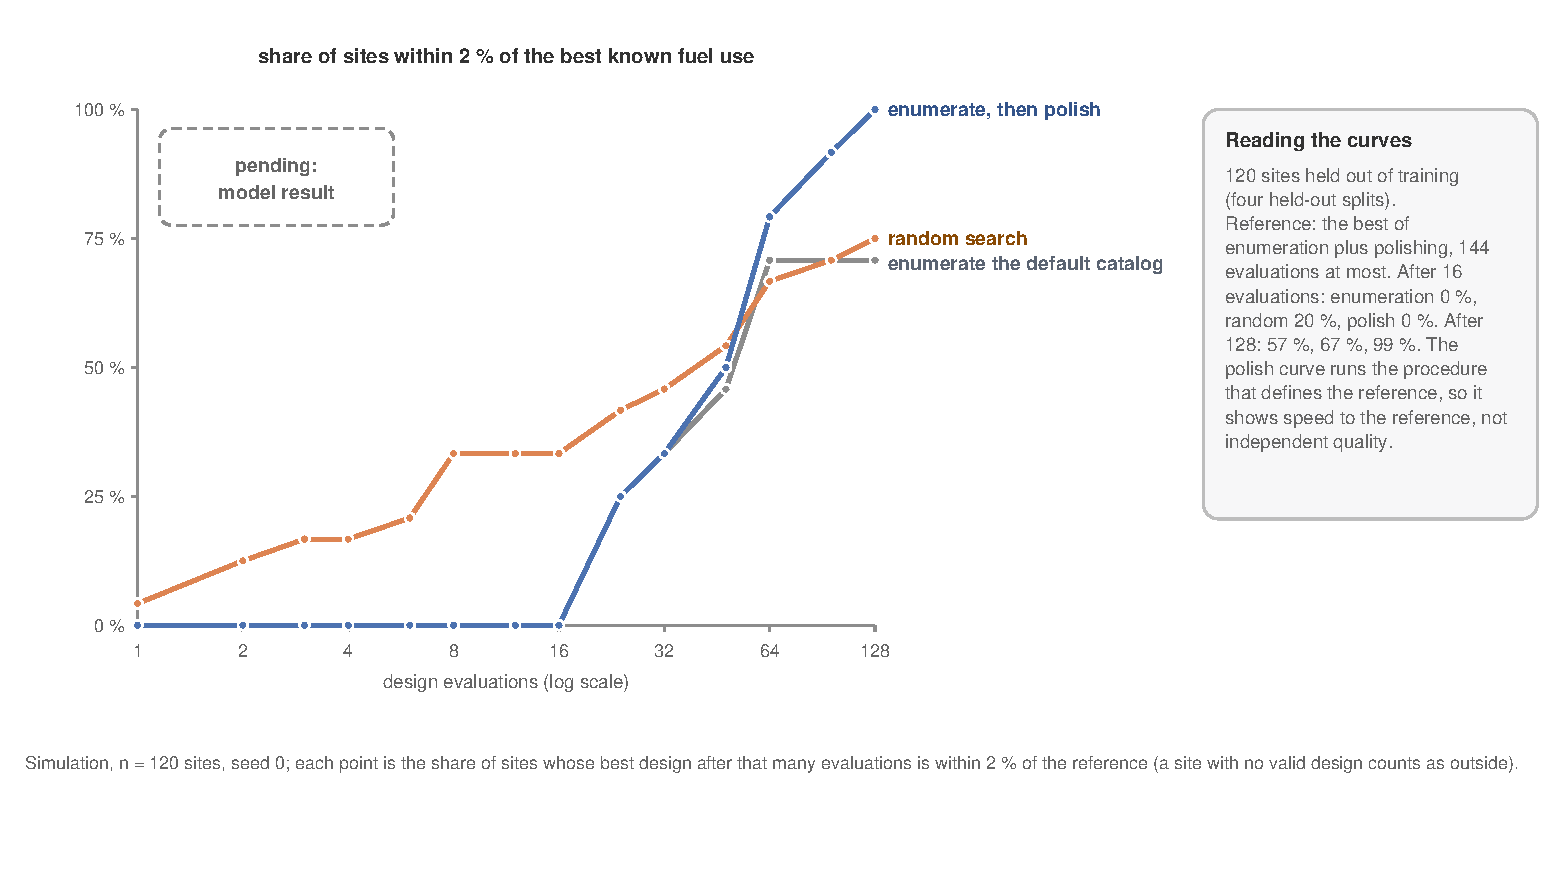
\includegraphics[width=\linewidth]{figures/pdf/fig_design_baselines.pdf}
\caption{Anytime curves of three non-model baselines on \val{des.n_sites} held-out sites (simulation): share of sites whose best design is within
\val{des.tolerance_pct}\% of the reference against the number of design evaluations (logarithmic scale). The reference is the enumerate-then-polish result. The trained-model curve is pending and
shown only as an empty box. Data: \texttt{assets/design\_baselines.json}.}
\label{fig:fig_design_baselines}
\end{figure}

\paragraph{Audit.}
On \val{audb.n_id} in-distribution and \val{audb.n_ood} held-out-topology plants, a fixed rule (raise the turbine inlet temperature by 10\%, or cut the engine loss fraction by 10\%) recovers
\val{audb.rule_gain_id_pct}\% of the best allowed gain on the in-distribution plants, where it is valid for \val{audb.rule_valid_id} of \val{audb.n_id}, and \val{audb.rule_gain_ood_pct}\% on the held-out engine and steam-ORC plants, where it is
valid for \val{audb.rule_valid_ood} of \val{audb.n_ood}. The best allowed change saves a median \val{audb.saving_median_id_pct}\% of fuel in-distribution (range \val{audb.saving_min_id_pct} to \val{audb.saving_max_id_pct}\%) and
\val{audb.saving_median_ood_pct}\% on the held-out topologies (\val{audb.saving_min_ood_pct} to \val{audb.saving_max_ood_pct}\%); exhaustive search over the allowed changes costs about \val{audb.search_evals_id} evaluations. For the prediction channel,
predicting no effect scores \val{audb.pred_zero_id} in-distribution and \val{audb.pred_zero_ood} held out, and predicting the mean relative effect of the other plants scores \val{audb.pred_mean_id} and \val{audb.pred_mean_ood}.

\paragraph{Ledger.}
A program that rebuilds each ledger line from the topology solves every row by construction, so there is no search baseline to report; the finding for this task is the symptom coverage of the faults (\cref{sec:ledger}).

\subsection{Simulator findings}\label{sec:findings}

These findings do not depend on a model. They characterize the simulator and the tasks under the assumed constants of \cref{tab:constants}.

\subsubsection{Feasibility mechanisms of the catalog}\label{sec:feasibility}

We evaluated the catalog at a 20~MW IT load (turbine exhaust about \val{mech.turbine_exhaust_K}~K, engine exhaust about \val{mech.engine_exhaust_K}~K), 25\,$^\circ$C ambient, 50\% relative humidity and
chilled water at 18 to 28\,$^\circ$C (\cref{tab:mech}; chilled fraction in steps of 0.05, wet tower, no grid import; one site, one point per entry). Five mechanisms follow.
\begin{itemize}[leftmargin=*,itemsep=1pt]
\item Exhaust-only recovery limits the engine. An engine with absorption cooling is valid up to \val{mech.engine_max_frac_pct}\% of the IT heat on the chilled loop, with a stack at \val{mech.engine_stack_K}~K; at \val{mech.engine_first_fail_pct}\%
the temperature-cross check fails, and at a chilled fraction of 1.0 the exhaust cannot supply the required duty. A turbine carries 100\% of the heat, with the stack still at \val{mech.turbine_100_stack_K}~K.
\item A single-stage ORC cannot use turbine exhaust: with none of the three fluids (valid for \val{mech.orc_turbine_valid} of \val{mech.orc_turbine_n}) can the evaporator accept an exhaust of about \val{mech.turbine_exhaust_K}~K without exceeding the vapor limit while leaving the stack above the floor.
\item On the engine, bottoming helps with the right fluid. Cyclopentane lowers fuel from \val{mech.eng_none_fuel_mw} to \val{mech.eng_cyc_fuel_mw}~MW (\val{mech.eng_cyc_saving_pct}\%) with \val{mech.eng_cyc_orc_net_mw}~MW of net ORC output, and toluene gives \val{mech.eng_toluene_fuel_mw}~MW; R245fa is infeasible because the exhaust is too hot for its vapor limit.
\item Dry rejection fails in heat. At 32\,$^\circ$C ambient an engine with a dry cooler and absorption cooling fails the temperature-cross check, while with a wet tower it is valid at \val{mech.amb305_wet_fuel_mw}~MW.
\item A water limit rules out wet towers: with a site limit of 0.5~kg/s, a wet tower fails the water check (the tower's make-up bound is \val{mech.water_wet_use_kg_s}~kg/s) and the dry-cooler plant is valid.
\end{itemize}

\begin{table}[tbp]
\centering
\begingroup\small\renewcommand{\arraystretch}{1.1}
\begin{tabular}{@{}rll@{}}
\toprule
Chilled fraction & Engine + absorption, wet tower & Turbine + absorption, wet tower \\
\midrule
0.3 & 48.4 MW, stack 667 K & 57.1 MW, stack 748 K \\
0.4 & 48.5 MW, stack 598 K & 57.3 MW, stack 710 K \\
0.5 & 48.7 MW, stack 529 K & 57.5 MW, stack 673 K \\
0.6 & 48.8 MW, stack 459 K & 57.7 MW, stack 635 K \\
0.7 & 49.0 MW, stack 388 K & 57.8 MW, stack 597 K \\
0.8 & infeasible & 58.0 MW, stack 559 K \\
0.9 & infeasible & 58.2 MW, stack 521 K \\
1.0 & infeasible & 58.4 MW, stack 483 K \\
\bottomrule
\end{tabular}\endgroup

\caption{Fuel use and stack temperature of engine and turbine plants with absorption cooling and a wet tower against the share of the IT heat carried by the chilled loop (20~MW IT load,
simulation, $n=2$ plants per row, assumed constants). ``Infeasible'' marks a plant that fails a hard check or cannot be sized. Data: \texttt{assets/mechanisms.json}.}
\label{tab:mech}
\end{table}

\Cref{fig:fig_design_feasibility} extends this to the whole catalog over \val{feas.n_cells} cells (chilled fraction and ambient temperature, \val{feas.n_specs} specifications each). Of the \val{feas.n_cells} cells, \val{feas.n_cells_none} (all at 283~K) have no valid design because the chiller's heat rejection (ambient plus approach)
is not above its evaporator temperature; free cooling is not modeled, so this is a limit of the model and not an engineering infeasibility. In the other \val{feas.n_cells_valid} cells the mean number of valid specifications is \val{feas.mean_valid} of \val{feas.n_specs},
the winners span \val{feas.n_winner_types} distinct configurations, the engine wins in \val{feas.win.engine_absorption} cells with absorption cooling and \val{feas.win.engine_electric} with electric cooling, and the turbine with absorption cooling wins in \val{feas.win.turbine_absorption}; in
\val{feas.n_ea_none} cells no engine and absorption design is valid.

\begin{figure}[tbp]
\centering
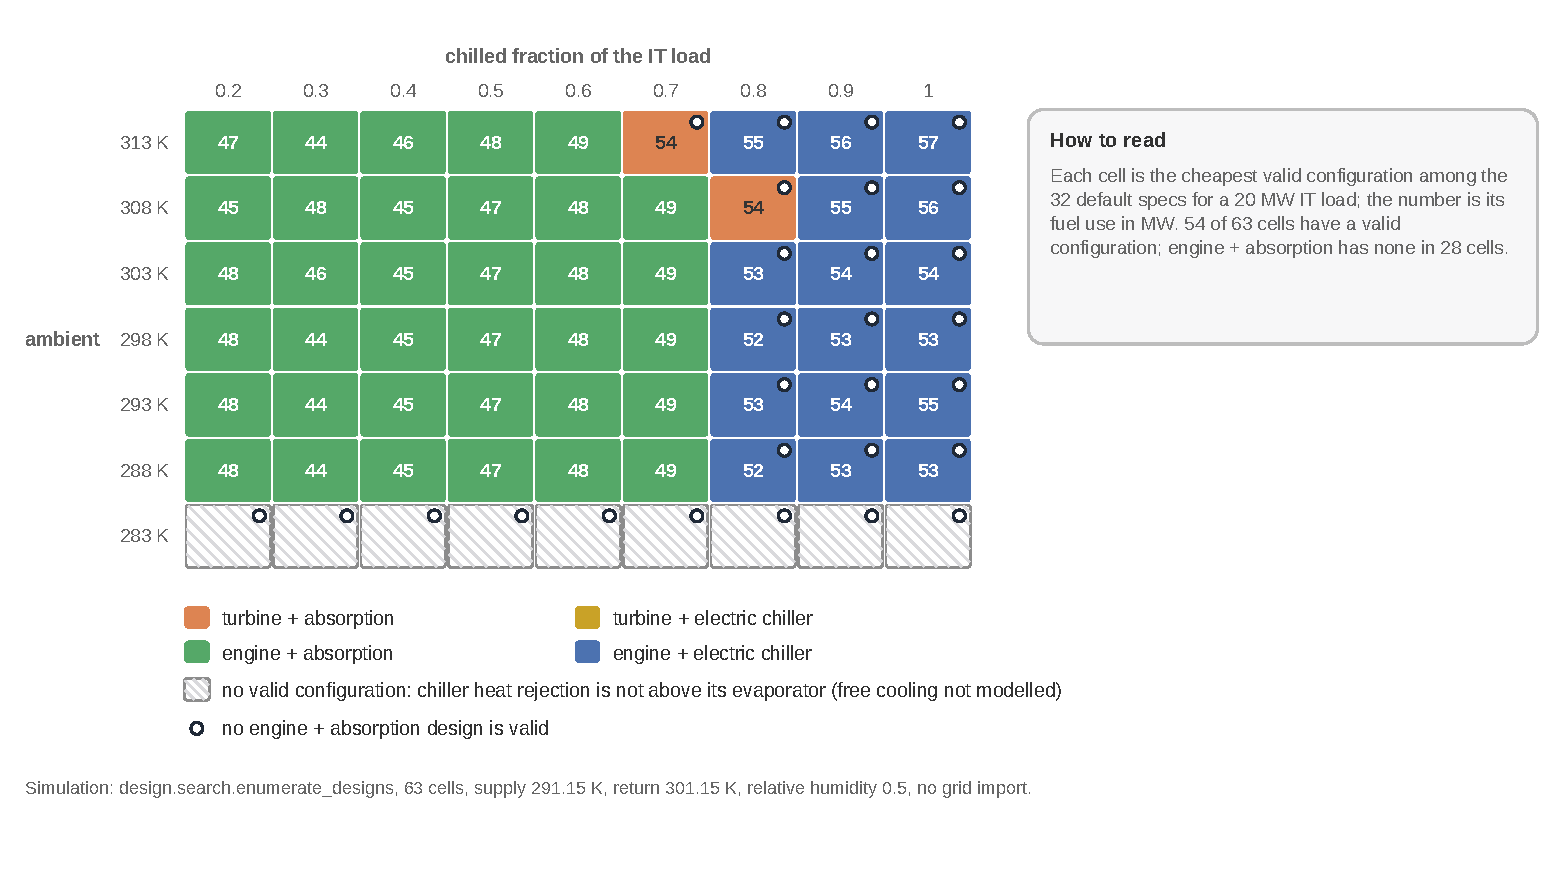
\includegraphics[width=\linewidth]{figures/pdf/fig_design_feasibility.pdf}
\caption{Best configuration family over chilled fraction and ambient temperature for a 20~MW IT load among the \val{feas.n_specs} default specifications (simulation, \val{feas.n_cells} cells). Numbers are fuel use in MW; hatched cells have no valid
configuration in the model; circles mark cells where no engine plus absorption design is valid. Data: \texttt{assets/design\_feasibility.json}.}
\label{fig:fig_design_feasibility}
\end{figure}

\subsubsection{First-law against second-law blame}\label{sec:audit}

A first-law ranking blames the component that dissipates the most energy to the surroundings. In one audited plant (\texttt{aud-0-00000}, a turbine plant with absorption cooling, fuel input \val{aud.ex_fuel_mw}~MW) it blames the heat rejector
\val{aud.ex_rej_id}, which dissipates \val{aud.ex_rej_energy_mw}~MW but destroys \val{aud.ex_rej_ed_mw}~MW of exergy, while exergy is destroyed in the prime mover \val{aud.ex_pm_id} (\val{aud.ex_pm_ed_mw}~MW, with \val{aud.ex_pm_energy_mw}~MW of energy dissipated) and, among the
other components, mostly in \val{aud.ex_top_id} (\val{aud.ex_top_ed_mw}~MW). Over plants, with the prime mover excluded because it was the largest destroyer in every plant, the first-law top choice is the true top destroyer in
\val{aud.fl_hits_id} of \val{aud.n_id} in-distribution plants (random order: \val{aud.rnd_top1_id_pct}\%) and \val{aud.fl_hits_ood} of \val{aud.n_ood} held-out-topology plants (\val{aud.fl_top1_ood_pct}\%, Wilson 95\% interval \val{aud.fl_ci_lo_ood_pct} to \val{aud.fl_ci_hi_ood_pct}\%; random
order \val{aud.rnd_top1_ood_pct}\%). In nDCG@3 the first-law ranking scores \val{aud.ndcg_fl_id} and \val{aud.ndcg_fl_ood} against \val{aud.ndcg_rnd_id} and \val{aud.ndcg_rnd_ood} for random order. The two samples disagree: in-distribution the first-law view is below random order on both metrics, while on the held-out diagrams it is clearly above them, so neither sample supports using energy dissipation as a proxy for exergy destruction. The Audit task therefore hides the destruction and asks the model to compute it; the model result is pending, and \cref{fig:fig_audit_first_vs_second_law} has no model bar.

\begin{figure}[tbp]
\centering
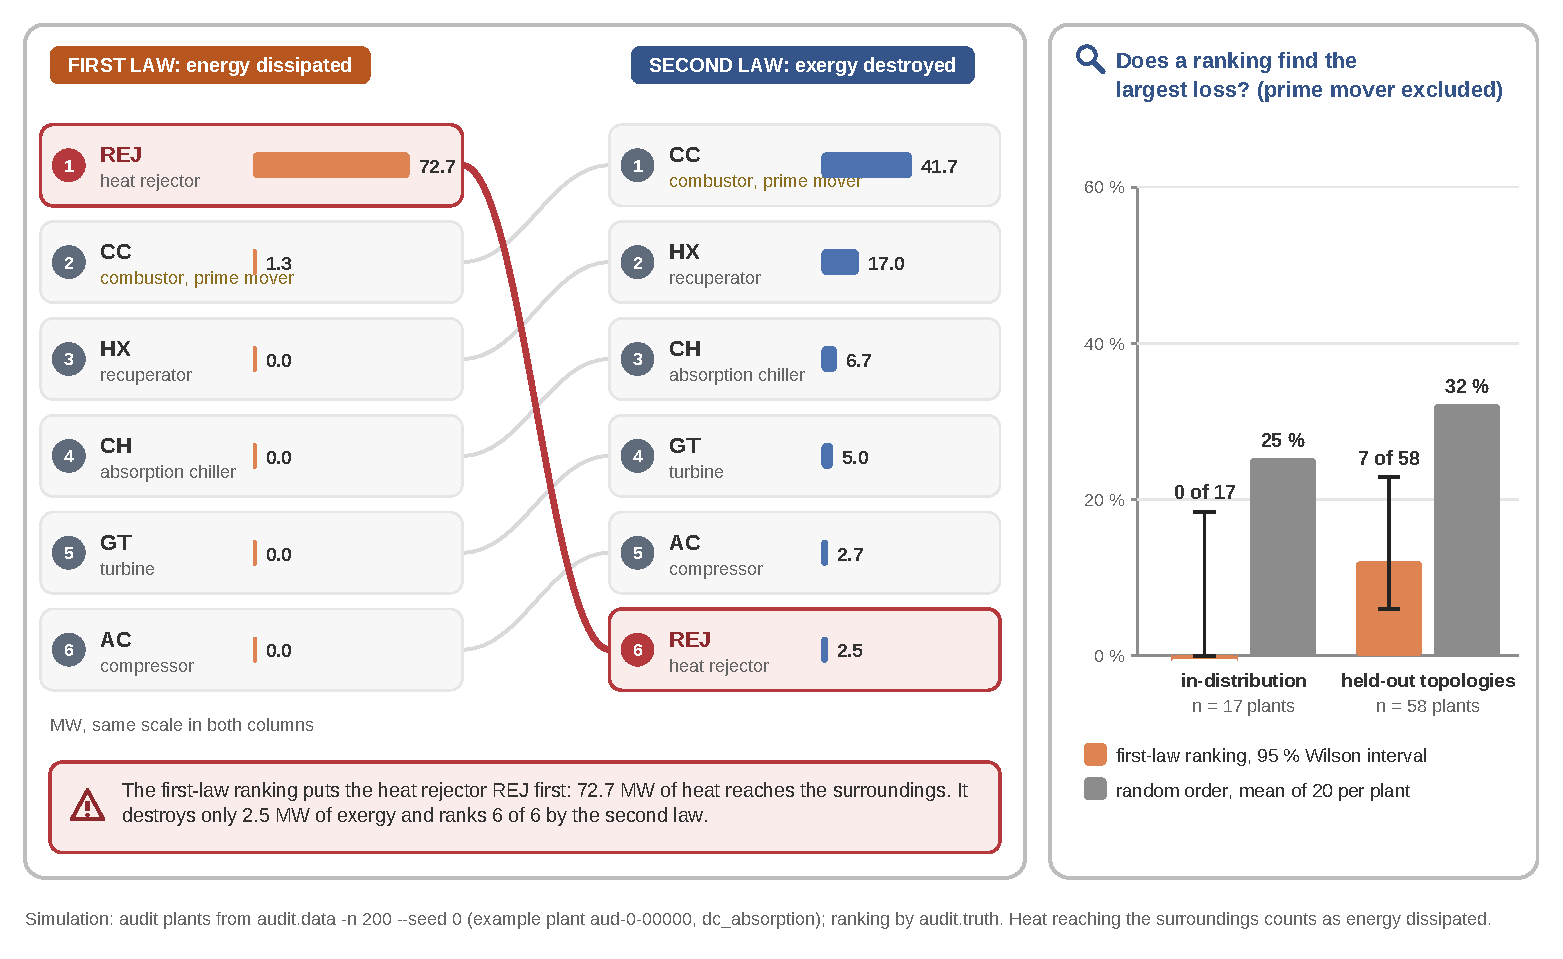
\includegraphics[width=\linewidth]{figures/pdf/fig_audit_first_vs_second_law.pdf}
\caption{First law against second law. Left: energy dissipated to the surroundings and exergy destroyed per component for one plant (simulation, $n=1$). Right: top-1 hit rate of the first-law ranking against random order, prime mover
excluded, on \val{aud.n_id} in-distribution and \val{aud.n_ood} held-out-topology plants (simulation, seed 0); whiskers are 95\% Wilson intervals. Data: \texttt{assets/audit\_first\_vs\_second\_law.json}.}
\label{fig:fig_audit_first_vs_second_law}
\end{figure}

\subsubsection{Symptom coverage of ledger faults}\label{sec:ledger}

For each of \val{led.n} generated ledger rows (\val{led.n_single} with one fault, \val{led.n_double} with two) we ask whether the ledger shows a second-law symptom: a closure residual or a negative exergy destruction.
\Cref{fig:fig_ledger_symptoms} gives the shares per fault type on the \val{led.n_single} single-fault rows. The result has a structure. A closure residual appears when a destruction line is wrong: in \val{led.comp_closure} of
\val{led.comp_rows} rows with a component-line fault. It does not appear for a fault in a stream line or in the constant: in \val{led.stream_closure} of \val{led.stream_rows} such rows, because an error in a stream value $E[x]$ or in $T_0$
enters the destruction lines of its producer and consumer with opposite signs and cancels in the sum (\cref{fig:fig_verifiers}); dropping a work term, by contrast, changes the closure residual by \val{led.demo_drop_work_mw}~MW in the example of the figure.
For those \val{led.stream_rows} rows the only symptom is a negative destruction, visible in \val{led.stream_neg} of them. Overall \val{led.any_pct}\% of the rows show at least one symptom and \val{led.none_pct}\% show none; the two constant faults (\texttt{t0\_celsius}, \texttt{t0\_offset}; \val{led.t0_celsius_n} rows each) show
no symptom at all. Parameter-range checks (V6) see \val{led.range_checks} of these faults, because the faults are in the equations and not in the plant parameters. A model that repairs the ledger therefore has to localize the fault from the text of the lines, not from the checks alone.

\begin{figure}[tbp]
\centering
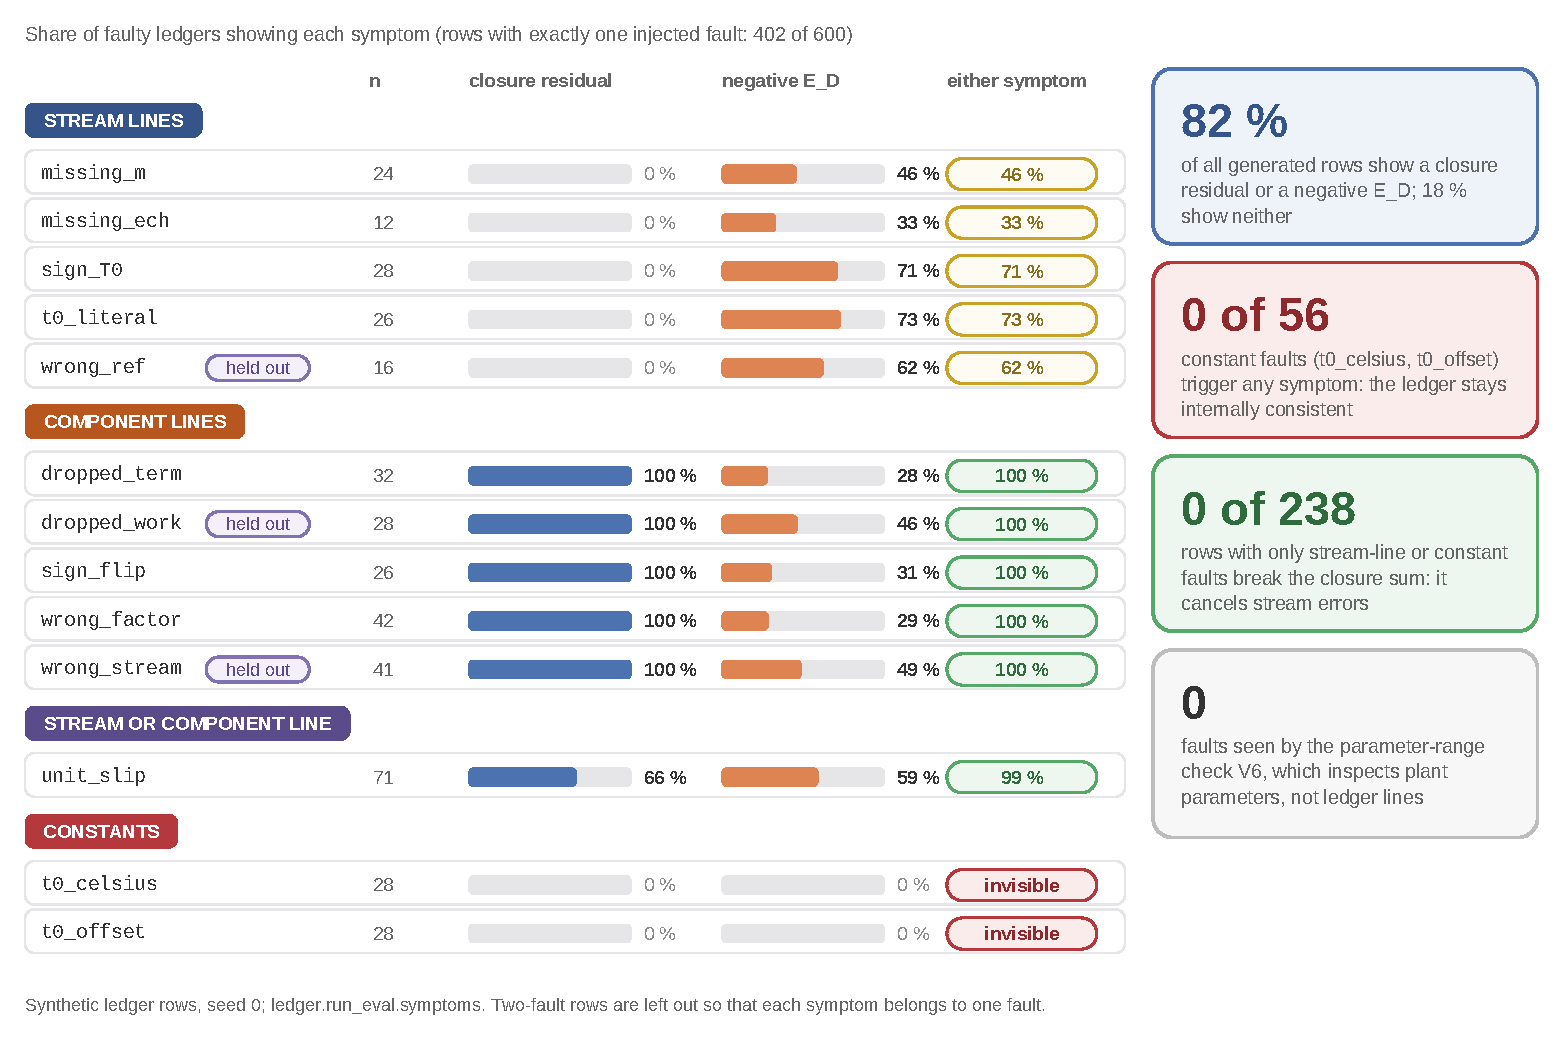
\includegraphics[width=\linewidth]{figures/pdf/fig_ledger_symptoms.pdf}
\caption{Symptoms of injected ledger faults: share of single-fault rows ($n=\val{led.n_single}$ of \val{led.n} generated rows, simulation, seed 0) showing a closure residual, a negative destruction, or either, by fault type and layer.
Stream-line and constant faults never break closure, and two constant faults show no symptom at all; parameter-range checks see none of these faults. Data: \texttt{assets/ledger\_symptoms.json}; the all-rows numbers are in \cref{app:faults}.}
\label{fig:fig_ledger_symptoms}
\end{figure}

\subsection{Current status: datagen and training}\label{sec:datagenstatus}

Datagen is incomplete, and Reza's directive of 2026-11-19 forbids starting SFT, GRPO or any training-based smoke test until every datagen item is built, audited and committed. The deterministic tool corpora currently hold 960 rows, built with \texttt{--limit 120} (240 per task), against a decided size of 4,800 rows (600 plants $\times$ 2 variants $\times$ 4 tasks). The plain A-slice is complete at 1,600 rows ($=\mathrm{round}(4{,}800\times0.3333)$, 400 per task). Only 32 verifier-accepted frontier tool traces exist, all from \texttt{google-gemini-3-8-flash} (40 attempts, five 429 errors, 32 accepted, \$0.842202 total); after sanitizing the provider \texttt{call\_id} wrapper the clean corpus has at most 7,268 tokens per row, all under the 8,192 gate. Luna, haiku, sol, opus, sonnet and gemini-4 traces are planned, not collected. Tiers are equal thirds per task in both training and test data, derived from \texttt{thermo\_agent/synth/tiers.py}, with the remainder to the higher tier. The test set \texttt{heldout\_v2} is frozen before scoring. Consequently there are no results for any SFT, GRPO or evaluation arm: the tables below are skeletons, and every value in \cref{sec:protocol} is planned, not measured.

\subsection{Model results}\label{sec:modelresults}

\Cref{tab:results,tab:comparison} are generated from the result JSON files listed in
\texttt{model\_results\_manifest.json} in the paper assets: one entry per arm, with its model family, mode (Z or H),
tool access and zero-shot flag. The protocol is pre-registered, but no arm has been scored: no trained checkpoint exists and the frontier arms are replays from \texttt{data/kaggle\_datasets/thermo-agent-eval-replays/}. Consequently both tables are skeletons (``pending'') and carry no measured model values, and the teacher acceptance statistics are pending (\cref{tab:corpusstatus}). When
the runs exist we will report all rows for the \texttt{heldout\_v2} test cells, with the intervals and tests of \cref{sec:protocol}; the 214-id \texttt{heldout} remains dev. No planned value is presented as a result.

\begin{table}[tbp]
\centering
\begingroup\scriptsize\setlength{\tabcolsep}{3pt}
\begin{tabular}{@{}p{1.3cm}p{4.4cm}p{1.9cm}p{1.9cm}p{1.9cm}p{1.9cm}@{}}
\toprule
Task & Model (full inference text) & \multicolumn{4}{c}{Metrics (per task; see text)} \\
\midrule
Repair & Qwen3.5-4B base & \todo{pending} & \todo{pending} & \todo{pending} & \todo{pending} \\
 & SFT, ground truth only & \todo{pending} & \todo{pending} & \todo{pending} & \todo{pending} \\
 & SFT, full corpus & \todo{pending} & \todo{pending} & \todo{pending} & \todo{pending} \\
 & SFT + GRPO & \todo{pending} & \todo{pending} & \todo{pending} & \todo{pending} \\
 & Teacher model \todo{name} & \todo{pending} & \todo{pending} & \todo{pending} & \todo{pending} \\
 & Other open model \todo{name} & \todo{pending} & \todo{pending} & \todo{pending} & \todo{pending} \\
\midrule
Design & Qwen3.5-4B base & \todo{pending} & \todo{pending} & \todo{pending} & \todo{pending} \\
 & SFT, ground truth only & \todo{pending} & \todo{pending} & \todo{pending} & \todo{pending} \\
 & SFT, full corpus & \todo{pending} & \todo{pending} & \todo{pending} & \todo{pending} \\
 & SFT + GRPO & \todo{pending} & \todo{pending} & \todo{pending} & \todo{pending} \\
 & Teacher model \todo{name} & \todo{pending} & \todo{pending} & \todo{pending} & \todo{pending} \\
 & Other open model \todo{name} & \todo{pending} & \todo{pending} & \todo{pending} & \todo{pending} \\
\midrule
Audit & Qwen3.5-4B base & \todo{pending} & \todo{pending} & \todo{pending} & \todo{pending} \\
 & SFT, ground truth only & \todo{pending} & \todo{pending} & \todo{pending} & \todo{pending} \\
 & SFT, full corpus & \todo{pending} & \todo{pending} & \todo{pending} & \todo{pending} \\
 & SFT + GRPO & \todo{pending} & \todo{pending} & \todo{pending} & \todo{pending} \\
 & Teacher model \todo{name} & \todo{pending} & \todo{pending} & \todo{pending} & \todo{pending} \\
 & Other open model \todo{name} & \todo{pending} & \todo{pending} & \todo{pending} & \todo{pending} \\
\midrule
Ledger repair & Qwen3.5-4B base & \todo{pending} & \todo{pending} & \todo{pending} & -- \\
 & SFT, ground truth only & \todo{pending} & \todo{pending} & \todo{pending} & -- \\
 & SFT, full corpus & \todo{pending} & \todo{pending} & \todo{pending} & -- \\
 & SFT + GRPO & \todo{pending} & \todo{pending} & \todo{pending} & -- \\
 & Teacher model \todo{name} & \todo{pending} & \todo{pending} & \todo{pending} & -- \\
 & Other open model \todo{name} & \todo{pending} & \todo{pending} & \todo{pending} & -- \\
\bottomrule
\end{tabular}\endgroup

\caption{Model results for the four tasks, generated from \texttt{model\_eval} reports: our checkpoints, frontier models (zero-shot, with inference text, with tools) and other models, with family, inference text and tool access recorded on each row. Metrics per task are listed in \cref{sec:protocol}.}
\label{tab:results}
\end{table}

\begin{table}[tbp]
\centering
\begingroup\scriptsize\setlength{\tabcolsep}{2pt}
\begin{tabular}{@{}p{3.4cm}p{1.8cm}p{2.2cm}p{1.4cm}p{6.2cm}@{}}
\toprule
Model & Family & Inference text & Tools & Metrics by task/split \\
\midrule
frontier\_zero & frontier & none & none & exact\_on\_deducible 0.37, first\_turn\_success 0.63, mean\_solves 1.33 \\
frontier\_zero & frontier & none & none & exact\_on\_deducible 0.33, first\_turn\_success 0.47, mean\_solves 0.77 \\
frontier\_zero & frontier & none & none & exact\_on\_deducible 0.10, first\_turn\_success 0.43, mean\_solves 1.13 \\
frontier\_zero & frontier & none & none & mean\_evals 0.17, mean\_gap\_pct 13.09, valid 0.17 \\
frontier\_zero & frontier & none & none & mean\_evals 0.30, mean\_gap\_pct 24.04, valid 0.20 \\
frontier\_zero & frontier & none & none & mean\_evals 0.07, mean\_gap\_pct 15.26, valid 0.07 \\
frontier\_zero & frontier & none & none & mean\_evals 0.10, mean\_gap\_pct 8.10, valid 0.10 \\
frontier\_zero & frontier & none & none & gain 0.00, pred 0.00, rank 0.09 \\
frontier\_zero & frontier & none & none & gain 0.00, pred 0.00, rank 0.03 \\
frontier\_zero & frontier & none & none & all\_correct 0.00, closure 0.03, exact 0.00 \\
frontier\_zero & frontier & none & none & all\_correct 0.00, closure 0.00, exact 0.02 \\
frontier\_zero & frontier & none & none & all\_correct 0.07, closure 0.07, exact 0.07 \\
frontier\_tools & frontier & none & tools & exact\_on\_deducible 0.37, first\_turn\_success 0.67, mean\_solves 1.07 \\
frontier\_tools & frontier & none & tools & mean\_evals 0.73, mean\_gap\_pct 16.37, valid 0.43 \\
frontier\_tools & frontier & none & tools & gain 0.00, pred 0.02, rank 0.13 \\
frontier\_tools & frontier & none & tools & all\_correct 0.77, closure 0.92, exact 0.77 \\
other\_model & domain-model & none & none & exact\_on\_deducible 0.22, first\_turn\_success 0.27, mean\_solves 0.67 \\
other\_model & domain-model & none & none & exact\_on\_deducible 0.50, first\_turn\_success 0.50, mean\_solves 1.00 \\
other\_model & domain-model & none & none & exact\_on\_deducible 0.17, first\_turn\_success 0.33, mean\_solves 0.73 \\
other\_model & domain-model & none & none & mean\_evals 0.17, mean\_gap\_pct 18.71, valid 0.17 \\
other\_model & domain-model & none & none & mean\_evals 0.30, mean\_gap\_pct 18.89, valid 0.30 \\
other\_model & domain-model & none & none & mean\_evals 0.17, mean\_gap\_pct 13.55, valid 0.17 \\
other\_model & domain-model & none & none & mean\_evals 0.23, mean\_gap\_pct 11.58, valid 0.23 \\
other\_model & domain-model & none & none & gain 0.00, pred 0.00, rank 0.00 \\
other\_model & domain-model & none & none & gain 0.00, pred 0.00, rank 0.00 \\
other\_model & domain-model & none & none & all\_correct 0.23, closure 0.53, exact 0.25 \\
other\_model & domain-model & none & none & all\_correct 0.13, closure 0.17, exact 0.17 \\
other\_model & domain-model & none & none & all\_correct 0.23, closure 0.35, exact 0.28 \\
\bottomrule
\end{tabular}\endgroup

\caption{Comparison axes: model family, inference text and tool access. The paired harness and tool columns isolate how much the physics tools help a frontier model, against the trained 4B and the non-model baselines.}
\label{tab:comparison}
\end{table}

\begin{figure}[tbp]
\centering
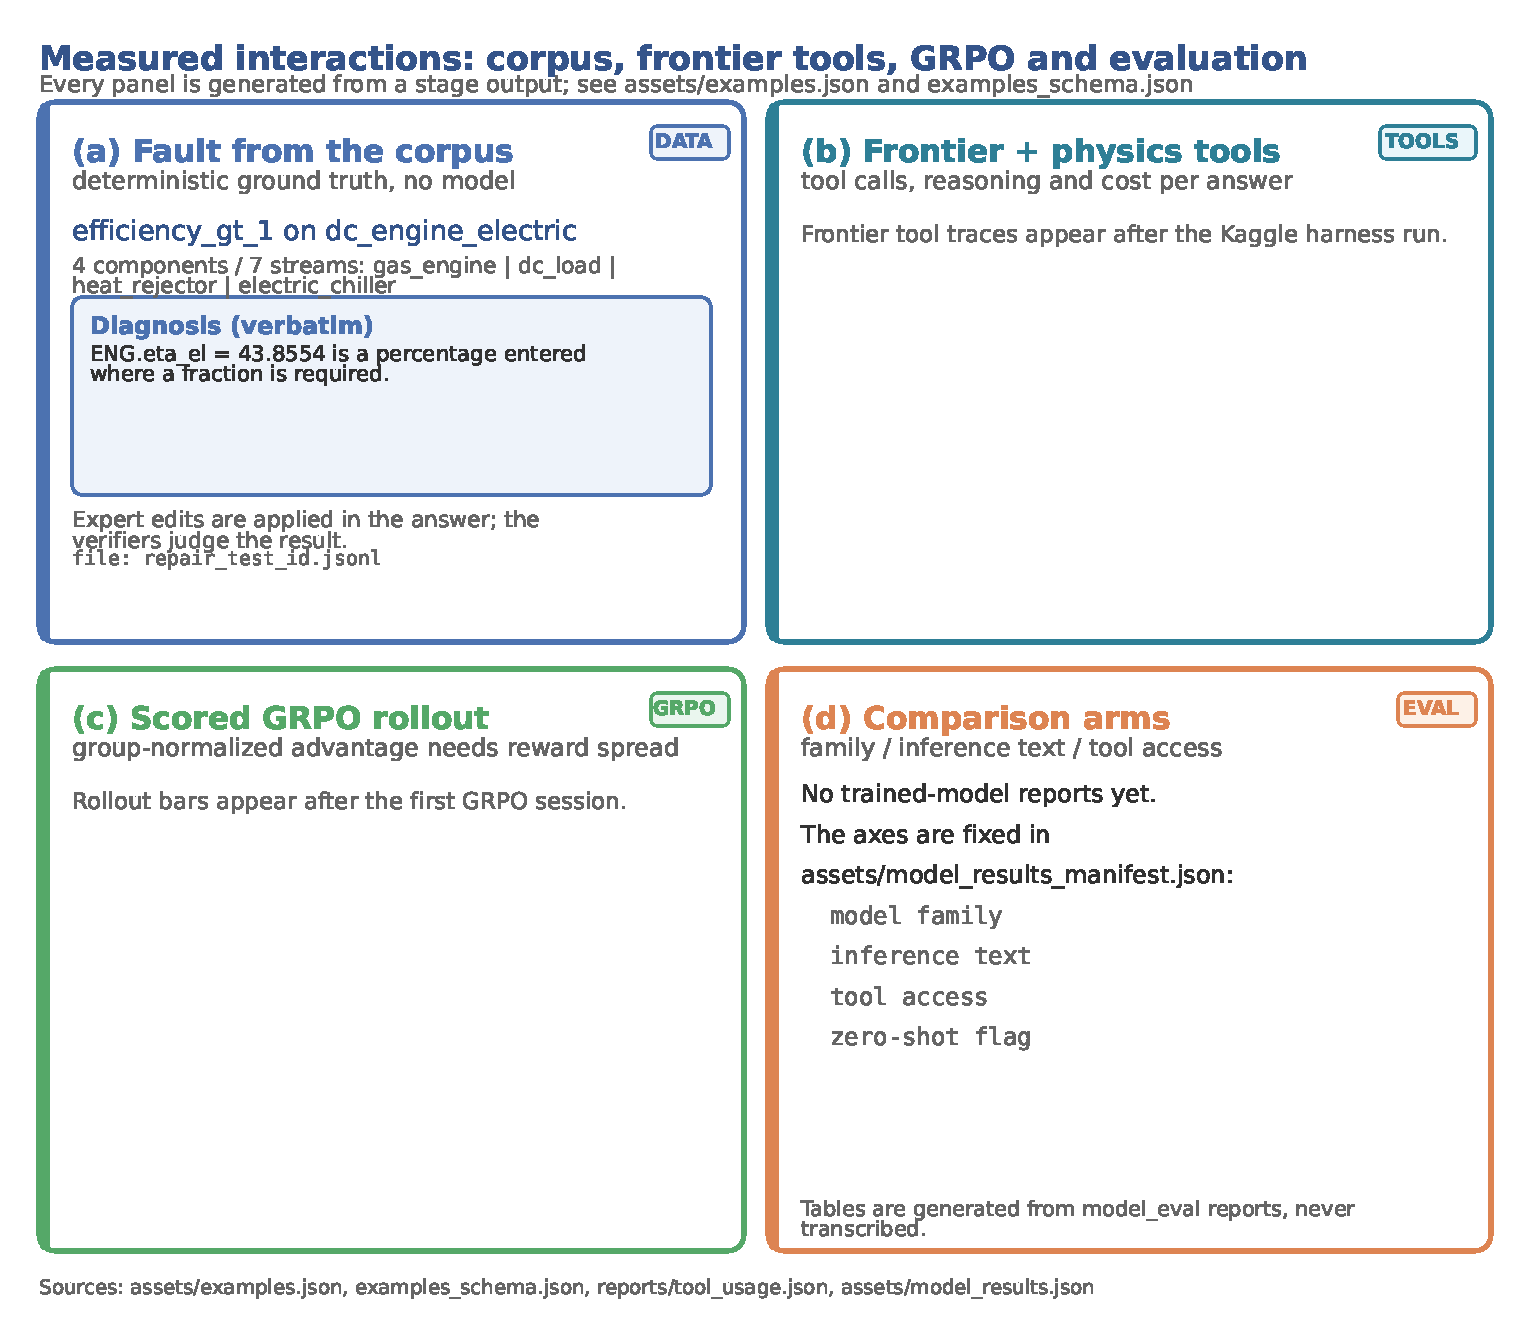
\includegraphics[width=\linewidth]{figures/pdf/fig_trace_walkthrough.pdf}
\caption{Interactions so far: a deterministic fault and its diagnosis, and a frontier model using our physics tools with recorded reasoning and cost (32 accepted traces from one model, replayed). The GRPO rollout and comparison panels are planned, not measured: they fill only after training runs, none of which has occurred. Every available element is copied from a stage output; the schema and selected examples are in \texttt{assets/examples.json} and \texttt{examples\_schema.json}. Regenerated by \texttt{figures\_from\_examples.py}.}
\label{fig:fig_trace_walkthrough}
\end{figure}

\subsection{Ablations}\label{sec:ablations}

\Cref{tab:ablation} lists the planned ablations: the inference text and the tool access on the held-out gas-engine diagrams (RQ2), the training corpus and the number of paraphrase variants per row (RQ7), the memory retrieval against no notes and random notes (RQ7), the reward channels and SFT against GRPO (RQ4), held-out diagram transfer (RQ3), an optional encoder-decoder variant, and ThermoQA accuracy before and after training (RQ6). All results are pending.

\begin{table}[tbp]
\centering
\begingroup\small\renewcommand{\arraystretch}{1.15}
\begin{tabular}{@{}p{4.3cm}p{6.1cm}p{2.9cm}l@{}}
\toprule
Ablation & Arms & Metric & Result \\
\midrule
Inference text on the held-out gas-engine diagrams & none / \texttt{AGENTS.md} / skills / both / both plus memory (base and trained) & success & \todo{pending} \\
Training corpus & ground truth only / plus architecture corpus / plus teacher traces / plus harness and memory text & success on held-out diagrams & \todo{pending} \\
Paraphrase variants per row & 1 / 3 / 20 or more & success on held-out faults & \todo{pending} \\
Memory retrieval & none / retrieved notes / random notes & success and acceptance rate & \todo{pending} \\
Reward channels & full / without site / without minimality / without grounding & success and valid share & \todo{pending} \\
SFT against GRPO from the base model & SFT only / SFT + GRPO / GRPO from base & success & \todo{pending} \\
Encoder-decoder variant (optional) & decoder-only / encoder-decoder & success & \todo{pending} \\
ThermoQA before and after training & base / SFT / SFT + GRPO & accuracy & \todo{pending} \\
\bottomrule
\end{tabular}\endgroup

\caption{Skeleton of the ablations. All results are pending.}
\label{tab:ablation}
\end{table}

\subsection{Reward diagnostics}\label{sec:rewarddiag}

Before any GPU time we asked how often a group of \val{rd.G} completions would have identical rewards, which carry no gradient under group-normalized advantages. The probe uses simulated policies that return the expert answer with probability $1-e$ and a damaged answer otherwise
(\val{rd.repair.groups} groups per task and level, seed 0; no model). At an error rate of 5\% the share of such groups is \val{rd.repair.zv_e5_pct}\% for Repair, \val{rd.design.zv_e5_pct}\% for Design, \val{rd.audit.zv_e5_pct}\% for Audit and \val{rd.ledger.zv_e5_pct}\% for Ledger repair;
at 10\% it is \val{rd.repair.zv_e10_pct}, \val{rd.design.zv_e10_pct}, \val{rd.audit.zv_e10_pct} and \val{rd.ledger.zv_e10_pct}\%; at 30\% it is \val{rd.repair.zv_e30_pct}, \val{rd.design.zv_e30_pct}, \val{rd.audit.zv_e30_pct} and \val{rd.ledger.zv_e30_pct}\%; and at 60\% it is
\val{rd.repair.zv_e60_pct}, \val{rd.design.zv_e60_pct}, \val{rd.audit.zv_e60_pct} and \val{rd.ledger.zv_e60_pct}\%. With the smaller group, equal groups are more frequent: at an error rate of 10\% the shares at a group of 8 are \val{rd8.repair.zv_e10_pct}, \val{rd8.design.zv_e10_pct}, \val{rd8.audit.zv_e10_pct} and \val{rd8.ledger.zv_e10_pct}\%. A task on which the SFT model is already accurate gives GRPO little to learn from, which is the reason for RQ3. A fresh reward evaluation costs
\val{rd.ledger.eval_ms}~ms for the ledger, \val{rd.repair.eval_ms}~ms for Repair, \val{rd.audit.eval_ms}~ms for Audit and \val{rd.design.eval_ms}~ms for Design per completion on the authoring machine (one CPU), so the reward is cheap relative to generation. \Cref{fig:fig_reward_signal} shows the curves.

\begin{figure}[tbp]
\centering
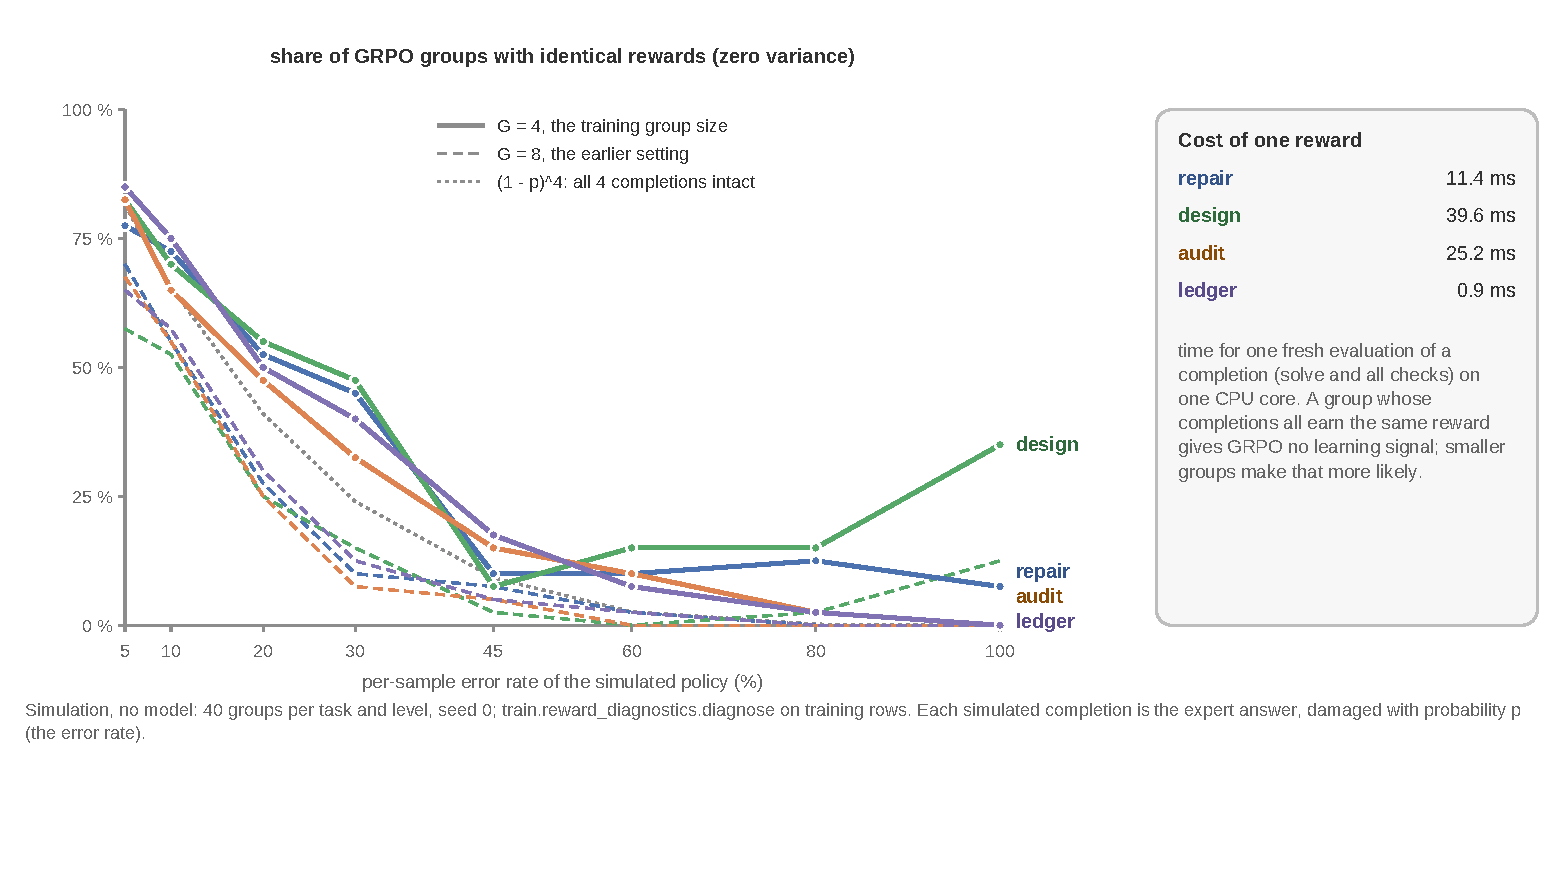
\includegraphics[width=\linewidth]{figures/pdf/fig_reward_signal.pdf}
\caption{Reward signal before any GPU time: share of GRPO groups whose completions all receive the same reward, against the per-sample error rate of a simulated policy, for each task, at the training group size of \val{rd.G} (solid) and at 8 (dashed), with the cost of one reward evaluation (simulated policies on synthetic data, no model; \val{rd.repair.groups} groups per task and level, seed 0). Data: \texttt{assets/reward\_signal.json}.}
\label{fig:fig_reward_signal}
\end{figure}

\subsection{What the remaining claims depend on}\label{sec:status}
The model-independent numbers in this paper are measured and reproducible from the checked-in generators and seeds: the verifier coverage, the baseline search costs, the feasibility and first-law findings, the reward diagnostics, and the data and corpus reports. The trained-model columns of \cref{tab:results,tab:comparison,tab:ablation} are pending, and the following runs are the only evidence that can fill them: the frontier teacher pass on Kaggle, local ingest and grading, the two-stage SFT/GRPO run on two T4 GPUs with resumable checkpoints, and the multi-arm evaluation of \cref{sec:protocol}. None of these runs has been executed. Until those runs exist we make no claim about the relative performance of the 4B model, the frontier arms or the other models, and \texttt{paper/assets/model\_results.json} contains the empty schema rather than numbers. The same rule applies to the cost columns: token prices are recorded when a Kaggle call happens, not estimated here.
